\section{Salmonella Method of Detection}
Current Salmonella detection methods that are available are listed in Figure \ref{CurrSalmDetecMetho} \cite{awangAdvancementSalmonellaDetection2021}. Most of these methods required expensive equipments, well-trained personal and no \textit{in-situ} testing \cite{shenBiosensorsRapidDetection2021,wangOverviewRapidDetection2021}. Furthermore, the time needed to detect the pathogen ranged between several hours to 4 hours  \cite{awangAdvancementSalmonellaDetection2021}.\\
\begin{figure}[h!]
    \centering
    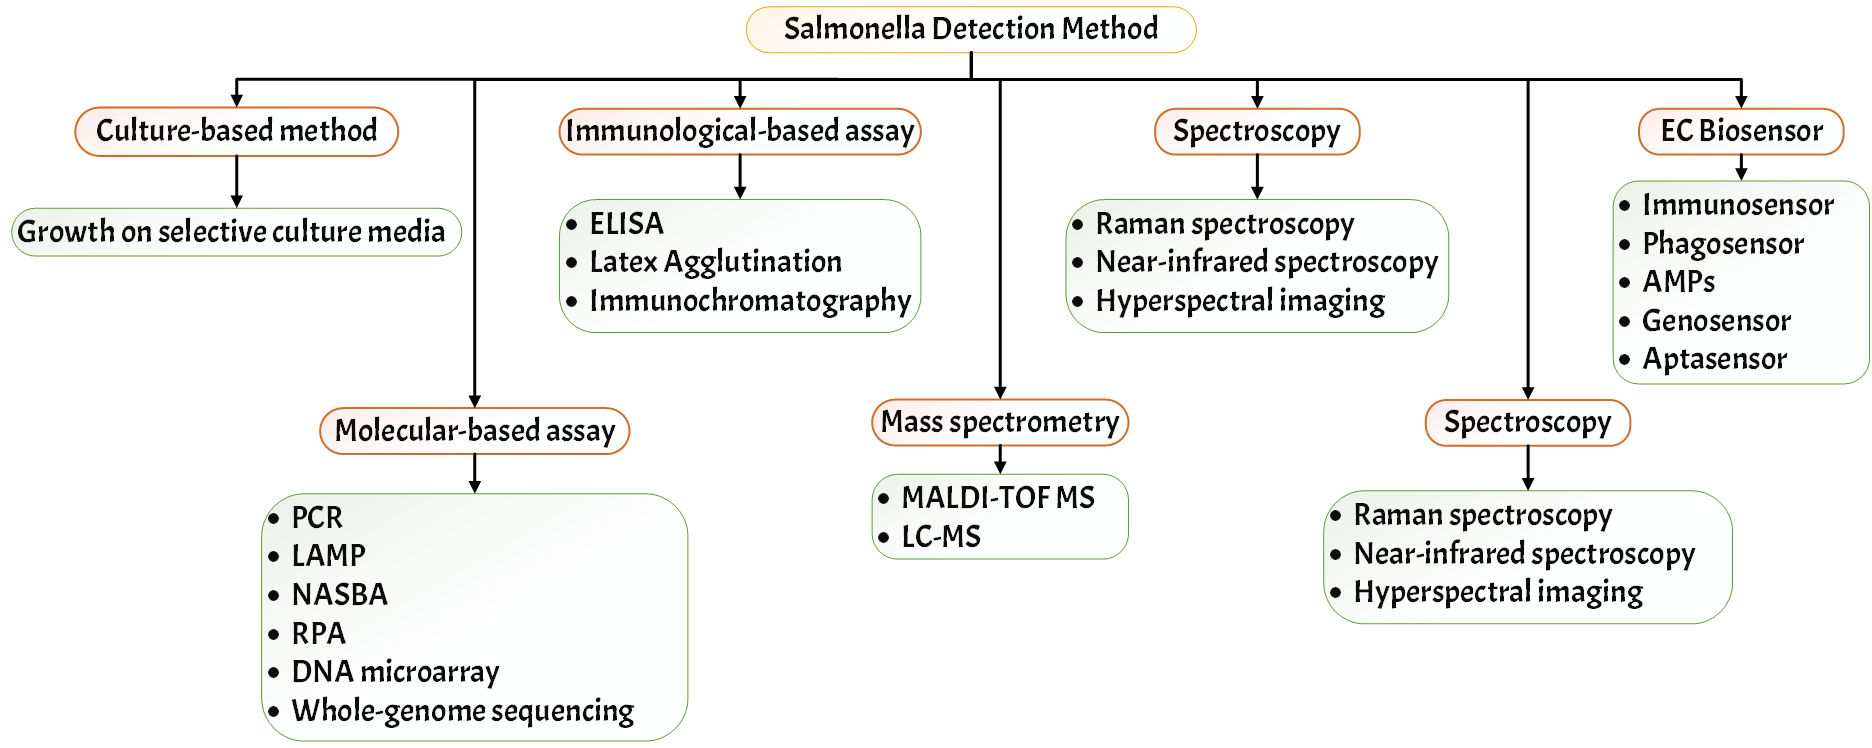
\includegraphics[width=\linewidth]{Figures/Awang_2021_Salmonella_Detection.png}
    \caption{Current available methods for Salmonella detection \\ (adapted from \cite{awangAdvancementSalmonellaDetection2021})}
    \label{CurrSalmDetecMetho}
\end{figure}

Due to these limitations, developments of rapid and sensitive detection methods of this particular pathogen has been researched to prevent another outbreak from occuring. The main concern is the modularity and compatibility with other techniques to have the sample to be tested on site and provide prelimninary finding before the sample is sent to the laboratory for more detail analysis.\newpage

One of the rapid detection methods in the biomedical space is DMF whereby droplets were generated from liquids in microliter (μL) and manipulated on an array of electrodes to perform protocols before the droplets are actuated to the sensing block for detection procedures.\\

This would allow parallel process to be conducted on the same electrodes, which helps in reducing waste and provide economical handling of the samples for on-site testing purposes \cite{agarwalDigitalMicrofluidicsTechniques2012}.\\